\documentclass[a4paper, 12pt]{scrreprt}

\usepackage[utf8]{inputenc}
\usepackage[T1]{fontenc}
\usepackage[acronym]{glossaries}
\usepackage{graphicx}
\usepackage{booktabs}
\usepackage{pdfpages}
\usepackage{hyperref}
\usepackage{listings}
\usepackage{tablefootnote}
\usepackage{verbatim}
\usepackage{multirow}
\usepackage{subcaption}
\usepackage{floatrow}
\usepackage[binary-units=true]{siunitx}
\usepackage{wasysym}
\usepackage{physics}
\usepackage{hyperref}

\usepackage[numbers]{natbib}


\title{Development of an ultra-wide band indoor positioning system}
\author{Antoine Albertelli}
\titlehead{{\Large Ecole Polytechnique Fédérale de Lausanne}\\
    Laboratoire de Systèmes Robotique (LSRO)\\
    Supervisor: Daniel Burnier
}

\begin{document}

\newacronym{imu}{IMU}{Inertial Motion Unit}
\newacronym{dmp}{DMP}{Digital Motion Processor}
\newacronym{uwb}{UWB}{Ultra Wide Band}
\newacronym{ekf}{EKF}{Extended Kalman Filter}
\newacronym{pan}{PAN}{Personal Area Network}
\newacronym{tof}{ToF}{Time of Flight}

\maketitle
\setcounter{tocdepth}{1}

\newcommand{\ieeepan}[0]{IEEE 802.15.4a}

\includepdf{abstract.pdf}
\tableofcontents

% TODO: Put each section in its own .tex
\chapter{Introduction}


Precise positionning is one of the key elements of a mobile robot.
It allows the software to take decisions and navigate to goals effectively.
Common approaches are inertial motion units or dead reckoning.

However those approaches tend to suffer from drift over time, due to their integration process.
They must be coupled with a reference system to correct the drift.
GPS can be used for this role, but does not work indoors.
We wanted to develop a new system that could enable indoor positioning of autonomous robots.

In recent year, \gls{pan} radio technologies have received more and more attention\cite{di2006uwb}, and standards for them have been appearing, mostly the \ieeepan{} standard.
Of particular interest are the \gls{uwb} systems, defined as having a bandwidth of more than \SI{500}{\mega\hertz} or 20\% of the center frequency\cite{uwb2006characteristics}.
From a communication point of view, \gls{uwb} is an interesting technology due to higher range and bandwidth.
However, it also enables new applications, including \gls{tof} calculation.

We wanted to use this \gls{tof} measurement to create an indoor positioning system for robots.
When looking at examples of positioning system for outdoors, a lot of them used a combination of GPS for global, noisy measurements and \gls{imu} (gyroscope, magnetometer and accelerometer) for local position data\cite{sporttracking,titterton2004strapdown}.
Commercial \gls{uwb} systems have also been used in conjunction with \gls{imu} sensors for greater accuracy\cite{corrales2008hybrid}.

\section{Working principle}

\begin{figure}[h!]
    \centering
    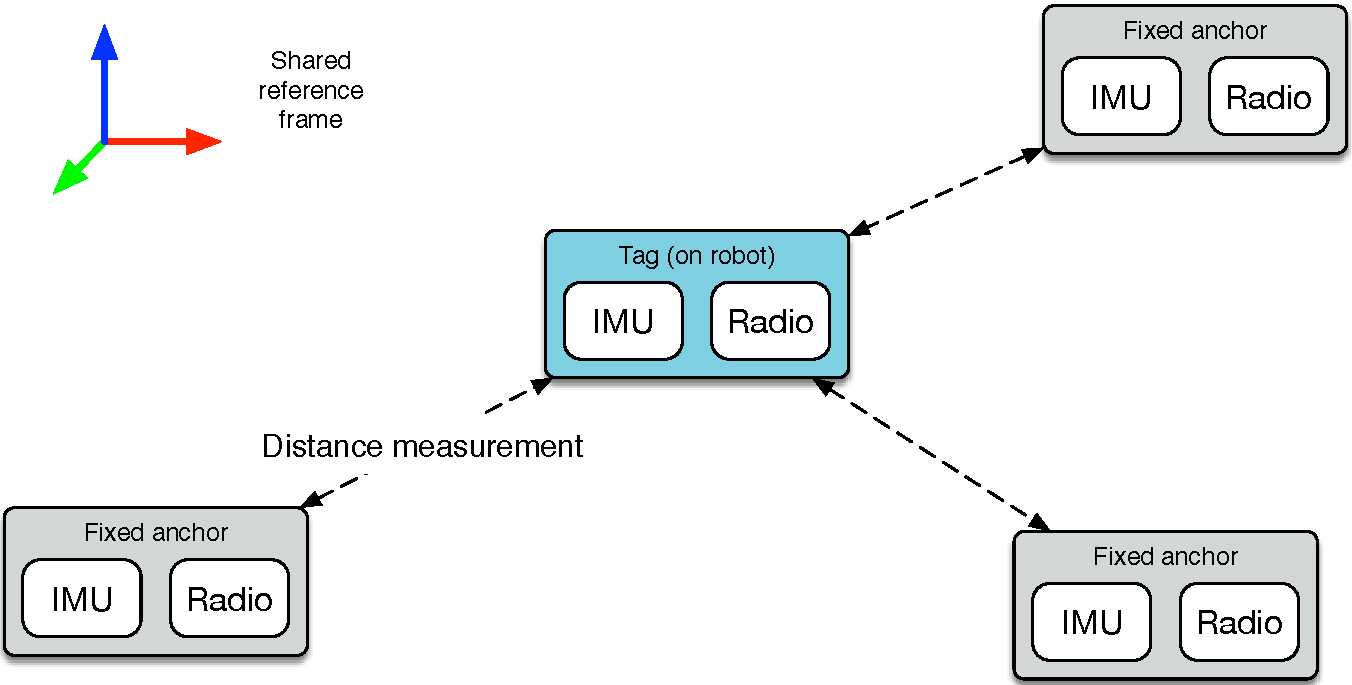
\includegraphics[width=0.6\textwidth]{figures/system.pdf}
    \caption{Overview of the system, showing one mobile robot (blue) and three fixed anchors (grey).}
    \label{fig:system}
\end{figure}

The complete system (Figure~\ref{fig:system}) is made of two types of nodes, tags and anchors.
The distance between each node is obtained by measuring the time of flight for a radio packet.
The tags are placed on each robot, and estimate their position using the \gls{imu} combined with the distance measurements to the anchors.
The anchors are at a reference position (fixed) and can be used by several tags.
A tag will always use all the available anchors and will be able to seamlessly switch in case a anchors is not in range anymore.

\section{Requirements}

Possible uses of this system include virtual reality and gaming, industrial automation, robotics contest, etc.
This work was done for use in robotics contest such as Eurobot or EPFL's internal contest.
However, we kept in mind the other applications and tried to avoid making choices that would make extension to other applications difficult.

For a robotics contest application, we decided on the following requirements:

\begin{enumerate}
    \item Ability to localize two robots at the same time.
    \item At least 3 anchors, uses more if more are available.
    \item The robots are moving in the 2D plane, but the anchors must not be in this plane.
    \item Reasonable positionning error ($\sigma=\SI{3}{\centi\meter}$).
\end{enumerate}

% TODO more requirements

\chapter{Hardware}

The board used in this project contains the following elements:

\begin{itemize}
    \item An Invensense MPU9250 \gls{imu}.
    \item A Decawave DW1000 \gls{uwb} transceiver.
    \item An STM32F411 microcontroller.
    \item USB and CAN interfaces.
\end{itemize}

\section{Inertial Motion Unit}

The MPU9250 is a 9 axis \gls{imu} made by Invensense\footnote{\url{https://www.invensense.com}}.
It was chosen because it combines an accelerometer, a gyroscope and a magnetometer in an easy to use package.
It is connected to the main microcontroller through an SPI bus.

An interesting feature of this device is the \gls{dmp}.
It is a low power co-processor that can be used for a variety of purpose, including orientation estimation, in which it directly outputs a quaternion.
Unfortunately, we found out that this feature is poorly documented by the manufacturer, making it impossible to use without reverse engineering.
Additionally, the \gls{dmp} cannot use the magnetometer data.
Therefore, we decided not to use it but to implement our own sensor fusion on top of raw sensor information.

\section{UWB transceiver}
The board contains an \gls{uwb} transceiver which combines a physical interface and a MAC.
It has several features useful for our application:
\begin{enumerate}
    \item \ieeepan{} compliant MAC which provides addressing features to avoid waking up on irrelevant traffic.
    \item High range, up to \SI{290}{\meter}.
    \item High accuracy timestamps for RX and TX of packets.
    \item High data rate (up to \SI{6.8}{\mega\bit\per\second}).
    \end{enumerate}

\chapter{Positioning algorithm}

\section{Parametric vs.\  non-parametric filter}

Parametric filters are filter which take assumptions on the distribution of the state.
The most common assumption is that the distribution is Gaussian.
Non parametric filters, on the other hand, can represent any distribution, and most importantly multi modal ones.

If the problem can be solved using a parametric filter, it is better, as they are computationally less expensive.
Since we are running the code on a small device with little computing power, it is important to take this into account.

Early on this project we decided to use an \gls{ekf},  which is one of the most common state estimator.
Like the Kalman filter, which assumes that the distributions of the state and noise are gaussian.
However, it works on non-linear dynamics, by approximating the non linearities via a first order Taylor expansion.

While the \gls{ekf} is easy to implement and lightweight computationally, it makes the assumption that the noises is distributed according to a normal law.
We verified this property for the measurement noise (see Section~\ref{sec:range_result}), but could only assume it for the process noise.

\section{Simulation}
\label{sec:simulation}

Testing the model's performance on the real system can be difficult.
First, implementing all the models in an embedded language like C or C++ is a tedious task.
Then, feeding the algorithm with recorded or generated measurements makes the results easier to compare and reproduce.
Therefore, we implemented a testing environment in Python.

Python allowed us to easily express high level mathematical objects.
For example, the Jacobian matrices are automatically computed using a symbolic math toolbox\footnote{Sympy: \url{http://www.sympy.org/}}, then converted to a numerical version.
Theoretically, it should even be possible to generate a C++ implementation from the symbolic representation, although that was not used in this project.
The framework allows us to create new \gls{ekf} models and test their performance in a matter of minutes.

\section{First model}

The goal of this model was to create the simplest thing that could possibly work.
It does not account for most issues, but was enough to start work on a simulator for the system.

To simplify the model, the following hypotheses are made:
\begin{enumerate}
    \item The robot moves in the 2D plane, i.e. its pose is described by $\left( x, y, \theta \right)$.
    \item The \gls{imu}'s internal motion processor already outputs $\theta$ (but it drifts).
    \item The \gls{imu} outputs the acceleration vector in body frame $\mathbf{a}^b$.
    \item The inertial frame is aligned with the world frame, i.e. the robot starts with $\theta=0$.
\end{enumerate}

The state contains the position and speed, in world frame:
\begin{equation}
    \mathbf{x} = \begin{pmatrix}x & y & \theta & \dot{x} & \dot{y}\end{pmatrix}^T
\end{equation}

\subsection{Motion model}

The first step is to transform the acceleration from body frame to world frame.

\begin{equation}
    \mathbf{a}^w = R(\theta) \mathbf{a}^b
\end{equation}

The state update equation, using the acceleration as control input

\begin{eqnarray}
    \dv{t} \mathbf{x} &=&
    \begin{pmatrix}
        \dot{x} & 
        \dot{y} &
        0 & % TODO: Maybe take it from acceleration ?
        \mathbf{a}^w_x &
        \mathbf{a}^w_y
    \end{pmatrix}^T \nonumber
    \\&=&
    \begin{pmatrix}
        \dot{x} \\
        \dot{y} \\
        0 \\  % TODO: Maybe take it from acceleration ?
        \cos(\theta) \mathbf{a}^B_x - \sin(\theta) \mathbf{a}^B_y \\
        \sin(\theta) \mathbf{a}^B_x + \cos(\theta) \mathbf{a}^B_y \\
    \end{pmatrix}
\end{eqnarray}

We can turn it into a discrete state update equation using the forward Euler method:

\begin{equation}
    \mathbf{x}_{t+1} = \mathbf{x}_t + \Delta_t \dv{t} \mathbf{x}
\end{equation}

\subsection{Measurement model}
In this model we have two different measurement functions.
The first one is the robot's heading, $\theta$, given by the \gls{dmp} or another attitute estimation algorithm.
\begin{equation}
    h_{\theta}(\mathbf{x}) = \theta
\end{equation}

The second type of measurement is the distance to the UWB anchors.
It is actually a family of functions; each beacon defines a measurement function.
This function is the distance to the position of the beacon, called $\mathbf{b}$.

\begin{equation}
    h_b(\mathbf{x}) = \sqrt{\left(\mathbf{x}_x - \mathbf{b}_x\right)^2 + \left(\mathbf{x}_y - \mathbf{b}_y\right)^2}
\end{equation}

\subsection{Simulation results}

\begin{figure}[h!]
    \centering
    \begin{subfigure}[t]{0.4\textwidth}
        \includegraphics[width=\textwidth]{models/simple_model_trajectory.pdf}
        \caption{Trajectory}
    \end{subfigure}%
    ~
    \begin{subfigure}[t]{0.4\textwidth}
        \includegraphics[width=\textwidth]{models/simple_model_error.pdf}
        \caption{Position error}
    \end{subfigure}
    \caption{Simulation results using the simple model.
        The simulated robot moves at \SI{0.17}{\meter\per\second}.
        The \gls{uwb} ranges arrive at \SI{10}{\hertz}, while the accelerometer information was integrated at \SI{200}{\hertz}.
        \label{fig:simple_model}
    }
\end{figure}

This simple model was converted to an \gls{ekf} model and implemented using the framework described in Section~\ref{sec:simulation}.
The noise characteristics of the ranging system were measured (see Section~\ref{sec:range_result}), while the accelerometer noise was taken from the datasheet.
The results can be seen in Figure~\ref{fig:simple_model}.

We think this behaviour is pretty suboptimal and that the \gls{ekf} could be better tuned.
However, we decided not to investigate this further, as this model required an absolute heading in the shared referene frame.
This is not easy to know: the magnetometers can give an absolute heading with respect to the Earth's magnetic frame, but we do not know the rotation between the north and the shared frame.
This led us to the creation of the next model.

\section{UWB only model}

This model was developped when I realized that the simple model had two important issues:

\begin{enumerate}
\item First, it supposed that we knew the rotation between the world frame and the earth magnetic frame, as the beacons' coordinates are in world frame, but the attitude of the robot is in earth magnetic frame.
\item The model had a lot of different variances to tune, making the tuning hard to do.
\end{enumerate}

This model removes those issues by relying only on the UWB radio ranging for measurement, and no prediction step.

\subsection{Model}

The state contains only the position of the robot.

\begin{equation*}
\mathbf{x} = \begin{pmatrix}x & y\end{pmatrix}^T
\end{equation*}


There is no information used for prediction, making the prediction function the identity:

\begin{equation}
\mathbf{x}_{k+1} = \mathbf{x}_{k}
\end{equation}

For the measurement, the UWB system gives us the distance $d$ to a beacon. The beacon's position $\mathbf{b}$ is known and assumed to be fixed.
Therefore the measurement model is given by Equation~\ref{eqn:uwb-only-measurement}.

\begin{equation}
h(\mathbf{x}, \mathbf{b}) = \sqrt{\left(x - b_x\right)^2 + \left(y - b_y\right)^2}
\label{eqn:uwb-only-measurement}
\end{equation}

\subsection{Tuning}

To compute the variance of the model, we estimate that the robot is moving at a constant speed of maximum $V_{max}$ between two measurements updates (which occurs at \(f_{UWB}\)).
Therefore, the maximum distance that a robot can do is given by Equation~\ref{eqn:travelled-distance}.

\begin{equation}
d = \frac{V_{max}}{f}
\label{eqn:travelled-distance}
\end{equation}

If we assume that \(d = 2 \sigma\), this means that our hypothesis is valid 97.5\% of the time, which is reasonable.
Therefore, the process variance can be estimated using Equation~\ref{eqn:variance}.

\begin{equation}
\sigma^2 = \left( \frac{V_{max}}{2 f} \right)^2
\label{eqn:variance}
\end{equation}

Assuming an update frequency of \SI{10}{\hertz} and a max speed of \SI{0.14}{\meter\per\second}, typical for a Thymio robot\cite{thymioweb}, we get a variance of $\sigma^2 = \SI{4.9e-5}{\meter\squared}$.


\subsection{Simulation results}

\begin{figure}[htpb]
    \centering
    \begin{subfigure}[t]{0.4\textwidth}
        \includegraphics[width=\textwidth]{models/uwb_only_trajectory.pdf}
        \caption{Trajectory}
    \end{subfigure}%
    ~
    \begin{subfigure}[t]{0.4\textwidth}
        \includegraphics[width=\textwidth]{models/uwb_only_error.pdf}
        \caption{Position error}
    \end{subfigure}
    \caption{
        Simulation results using only \gls{uwb} range information with 3 beacons.
        The simulated robot moves at \SI{0.17}{\meter\per\second}.
        The beacon distances were updated at \SI{10}{\hertz}.
        \label{fig:uwb_only}
    }
\end{figure}


\section{Differential measurement}

Out of curiosity, we also tried to implement a model where the robot would embed two \gls{uwb} modules separated by a known distance.
This should allow for a better precision, as well as measuring the heading of the robot.
We made the following assumptions:

\begin{enumerate}
    \item Robot moves in the 2D plane
    \item Gyro in the yaw axis
    \item  Gyroscope has constant bias ($b_\omega$) and random noise.
    \item \gls{uwb} receivers are separated by a fixed distance $d$.
\end{enumerate}

The state vector of the robot contains the position, speed and heading.
It also contains a constant term for the gyro bias, used to model the noise on the bias.


\begin{equation}
\mathbf{x} = \begin{pmatrix} x & y & \dot{x} & \dot{y} & \theta & b_{\omega} \end{pmatrix}^T
\end{equation}

\subsection{Model}

The prediction step uses outputs of the accelerometer (in body frame) and the angular rate as control inputs:

\begin{equation}
\mathbf{u} = \begin{pmatrix}
    a_x\\
    a_y\\
    \omega
\end{pmatrix}
\end{equation}

The differential equation governing the state evolution is therefore:

\begin{equation}
\mathbf{\dot{x}} = \begin{pmatrix}
\dot{x}\\
\dot{y}\\
\cos(\theta) a_x - \sin(\theta) a_y \\
\sin(\theta) a_x + \cos(\theta) a_y \\
\omega - b_{\omega}\\
0
\end{pmatrix}
\end{equation}

Using forward Euler integration we get:

\begin{equation}
\mathbf{x}_{k+1} = \mathbf{x}_{k} + \Delta_t \mathbf{\dot{x}} = \mathbf{g}\left(\mathbf{x}_{k}, \mathbf{u}_k\right)
\end{equation}

For the measurement step, the UWB system gives us the distance $d$ to a beacon.
The beacon's position $\mathbf{b}$ is known and assumed to be fixed.

We first compute the position of each UWB receiver. Receiver $n$ is assumed to be at position $\mathbf{x}_{UWB,n}^R$ in robot frame.

\begin{equation}
\mathbf{x}_{UWB,n}^W = \mathbf{x}_{robot}^W + \begin{pmatrix}
\cos \theta & - \sin \theta \\
\sin \theta & \cos \theta
\end{pmatrix} \mathbf{x}_{UWB,n}^R
\end{equation}

Then the measurement model is:

\begin{equation}
h_n(\mathbf{x}, \mathbf{b}) = \sqrt{(x_{UWB,n}^W - b_x)^2 + (y_{UWB,n}^W - b_y)^2}
\end{equation}

\subsection{Simulation results}

\begin{figure}[h!]
    \centering
    \begin{subfigure}[t]{0.4\textwidth}
        \includegraphics[width=\textwidth]{models/differential_model_trajectory.pdf}
        \caption{Trajectory}
    \end{subfigure}%
    ~
    \begin{subfigure}[t]{0.4\textwidth}
        \includegraphics[width=\textwidth]{models/differential_model_error.pdf}
        \caption{Position error}
    \end{subfigure}

    \begin{subfigure}[t]{0.4\textwidth}
        \includegraphics[width=\textwidth]{models/differential_model_angle.pdf}
        \caption{Angle estimation}
    \end{subfigure}

    \caption{Simulation results using the differential model.
        The simulated robot moves at \SI{0.17}{\meter\per\second}.
        The \gls{uwb} ranges arrive at \SI{10}{\hertz}, while the accelerometer information was integrated at \SI{200}{\hertz}.
        \label{fig:differential_model}
    }
\end{figure}


\section{Attitude estimation}

While an attitude estimator could be implemented directly in the \gls{ekf}, we chose to use a Madgwick estimator instead.
This estimator is a relatively novel technique based on gradient descent.
It is typically as accurate as an \gls{ekf}, while being less computationally expensive\cite{madgwick2011estimation}.

The Madgwick filter takes as inputs the measurements of linear acceleration, angular rates and magnetic fields.
It then computes the optimal state estimation, and returns it as a quaternion.
We used the reference implementation\cite{madgwick2011estimation} which was already suitable for microcontroller use.

\chapter{Implementation}

\section{UWB beacons protocol}

\subsection{Design principles}

\begin{enumerate}
    \item The protocol should require as little state as possible to be stored on the participating beacons.
        State synchronisation between several systems is a common source of error and bugs.
    \item We want to maximize the measurement frequency, which means we should have a measurement simple with as little packets as possible.
    \item To avoid waking up the microcontroller, the MAC layer integrated in the \gls{uwb} module must be leveraged as much as possible.
    \item The same radio link used for range measurement will also be used as a general purpose link to transmit data between nodes.
\end{enumerate}

\subsection{Time measurement}

\begin{figure}[h]
    \centering
    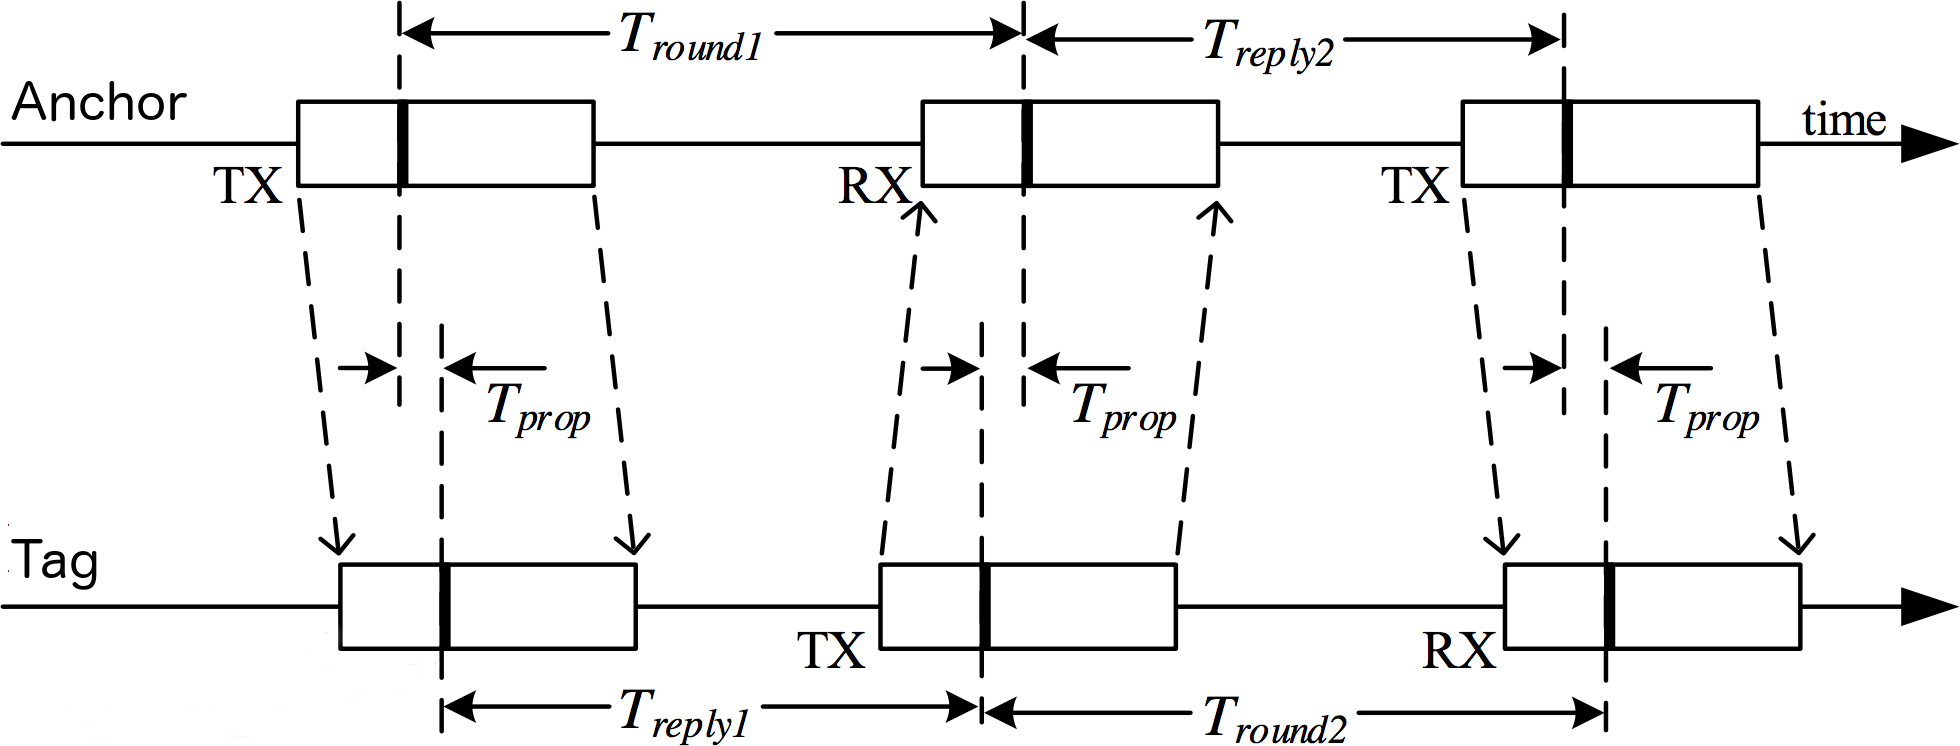
\includegraphics[width=0.8\textwidth]{figures/ranging_protocol.png}
    \label{fig:ranging_protocol}
    \caption[Ranging protocol]{Messages in a time measurement interaction. Source:~\cite{dw1000manual}}
\end{figure}

The time measurement protocol is composed of a sequence of 3 messages.
To initiate a measurement sequence, an anchor broadcasts a measurement advertisement message to the broadcast address (0xFFFF).
Tags may respond with a measurement reply message.
Finally, the anchor sends a measurement finalization message and the tag computes the ranging solution:

\begin{equation}
T_{prop} = \frac{T_{round,1} \cdot T_{round,2} - T_{reply,1} \cdot T_{reply,2}}{T_{round,1} + T_{round,2} + T_{reply,1} + T_{reply,2}}
\label{eqn:ranging}
\end{equation}

The timing information is then converted to a distance by multiplying by the speed of light ($c$).

This 3-way ranging scheme works because transceivers can be programmed to send a frame at a given time.
Therefore, $T_{reply,2}$ can be included in the final message.

Some random implementations notes:

\begin{enumerate}
    \item Use 802.15.4 MAC to enable hardware filtering.
    \item Sequence number field will be hacked to store packet type in it instead.
    \item All numbers in payload are sent in network byte order (most significant byte first).
    \item All timestamps in messages are in DW1000 units and without a shared reference.
\end{enumerate}

\paragraph{Measurement advertisement}
A measurement advertisement message has a sequence number of 0.
It is sent by an anchor to the broadcast address (0xFFFF).
It only contains the TX timestamp as a 40 bit unsigned integer ($T_{tx,1}$).

\paragraph{Measurement reply}
A measurement reply message has a sequence number of 1.
It is sent by a tag and contains the timestamps of all events so far ($T_{tx,1}$, $T_{rx,1}$ and $T_{tx,2}$)

\paragraph{Measurement finalization}
Finally, the measurement finalization has a sequence number of 2.
It is sent by the anchor and contains the content of the previous message plus the new timestamps ($T_{rx,2}$, $T_{tx,3}$).

Once the tag received the last message, it can compute the ranging solution using Equation~\ref{eqn:ranging} with the following informations:
\begin{eqnarray*}
    T_{round,1} &=& T_{tx,1} - T_{rx,2} \\
    T_{reply,1} &=& T_{rx,1} - T_{tx,2} \\
    T_{round,2} &=& T_{tx,2} - T_{rx,3} \\
    T_{reply,2} &=& T_{rx,2} - T_{tx,3} 
\end{eqnarray*}



\subsection{Antenna delay calibration}
In order to obtain correct range readings, we should take in account the delay created by antenna transmission.
This delay should be calibrated as it will be different for each design \cite{dw1000manual}.
To do it, we simply measured the distance reported by the modules over a known range (averaged on N samples).
The antenna delay ($\Delta_T$) can then be computed by equation~\ref{eqn:delay-calibration}.

\begin{equation}
    \Delta_T = \frac{d_{measured} - d_{real}}{2\cdot c}
    \label{eqn:delay-calibration}
\end{equation}

On our system, this value was found to be about 32905~DW1000's internal units (\SI{64.3}{\micro\second}).

\chapter{Results}

\section{Range measurement}
\label{sec:range_result}

% TODO test precision and recall

\begin{figure}[h]
    \centering
    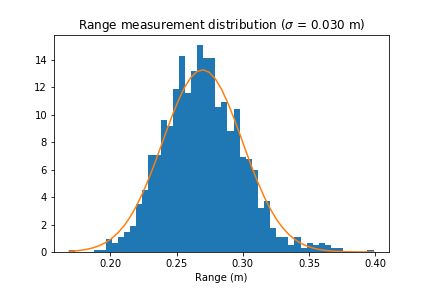
\includegraphics[width=0.6\textwidth]{experiments/range_noise.pdf}
    \caption{Distribution of the range measured by the \gls{uwb} module in the optimal orientation.
        The corresponding gaussian fit is shown.
        We see that the error is pretty much normally distributed.
    }
    \label{fig:range_noise}
\end{figure}

% TODO: Impact of antenna orientation
% TODO: Impact of preamble length

\chapter{Future work}
\appendix
\chapter{Hardware schematic}

The following schematic is the one of the board used during this project.
However, several flaws were discovered and should be corrected before a new batch is produced.

\begin{itemize}
    \item There is currently no way to use the USB bootloader built in the microcontroller.
        This makes updating the board's firmware harder, as it requires a specialized debug adapter.
        Adding a button on pin BOOT0 would allow the user to enter bootloading mode as well as serving as a general purpose button.
    \item The reset pin of the \gls{uwb} module is connected to a pin used by the USB module of the microcontroller.
        Although one should be able to disable this pin by software, we could not make it work and had to cut a connection on the board.
\end{itemize}

All design documents and related issues can be found on the board's Github repository\footnote{\url{https://github.com/cvra/uwb-beacon-board/}}.


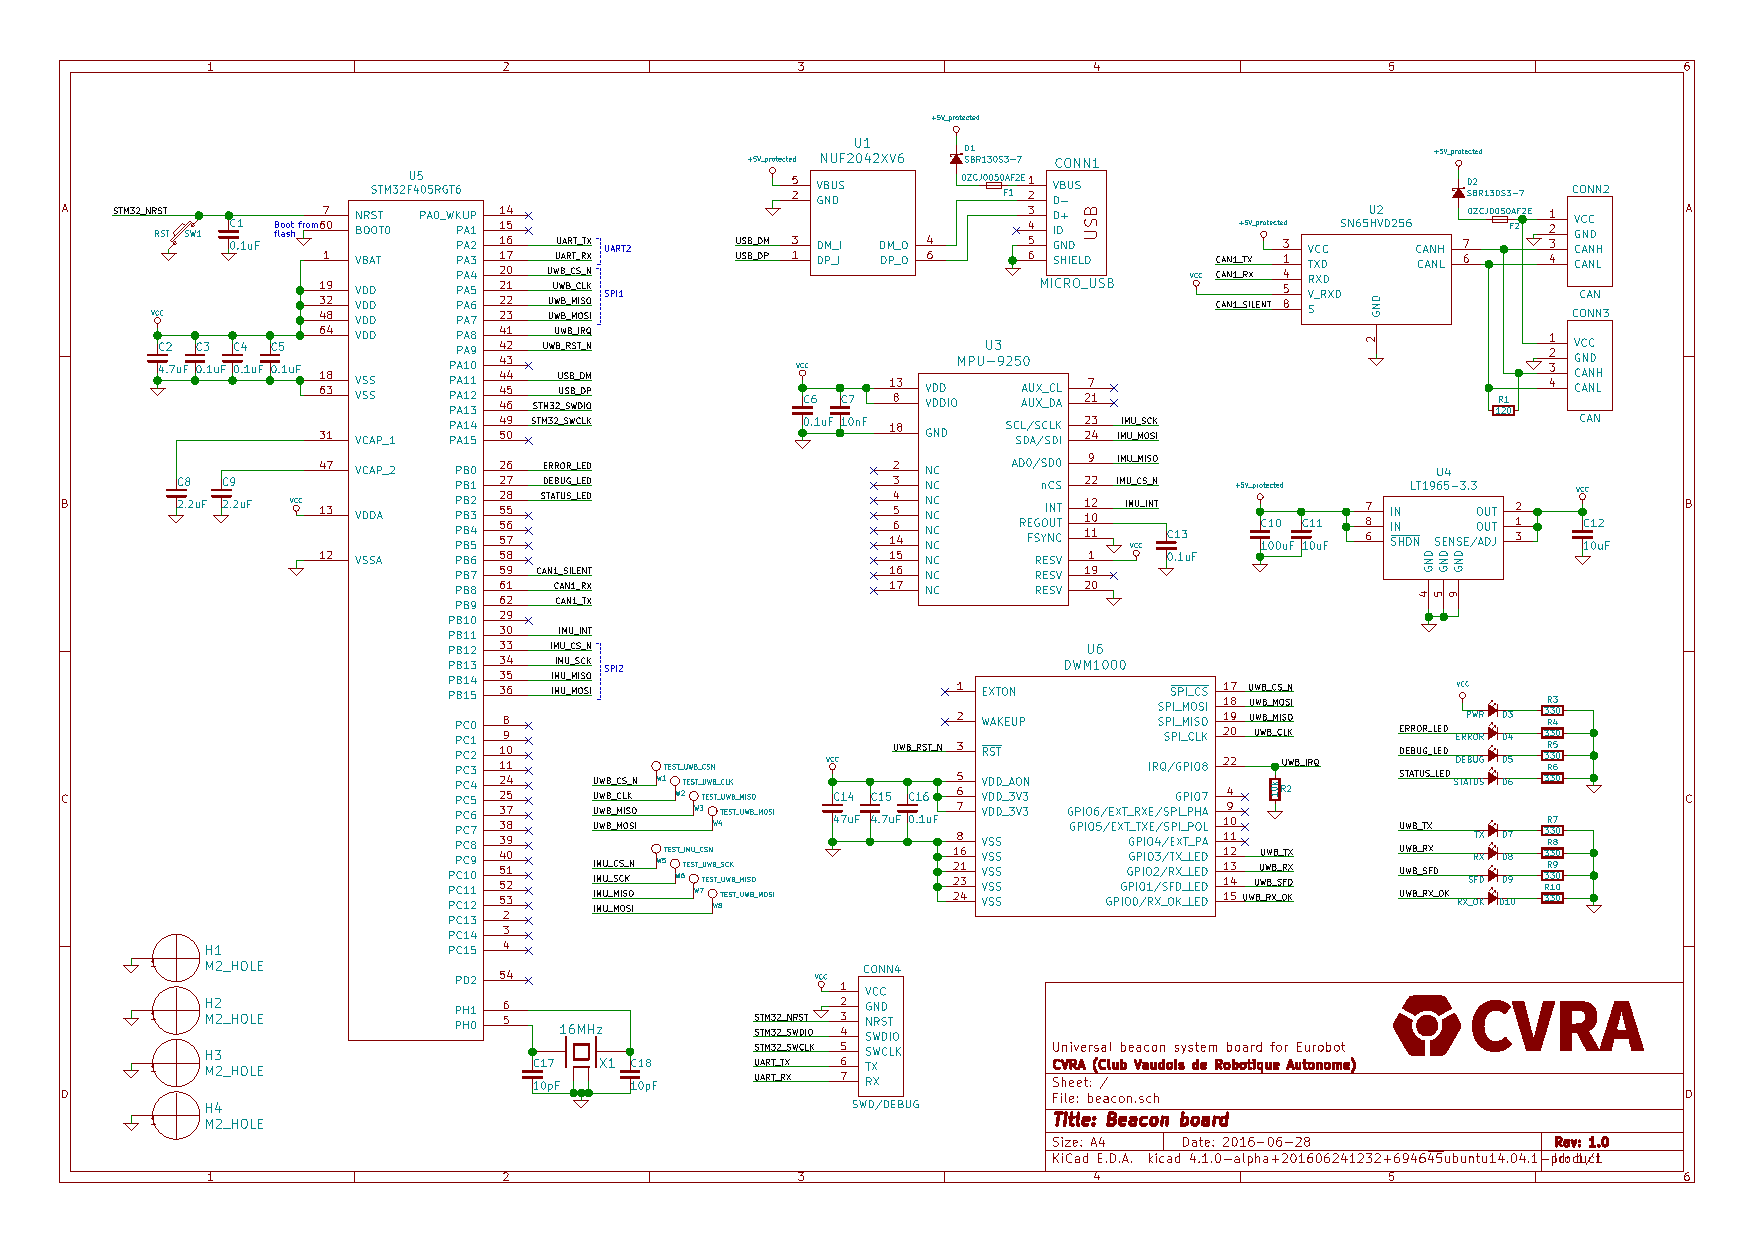
\includepdf[landscape=true]{figures/board_schematic.pdf}

\chapter{User manual}


\clearpage
\nocite{*} % tells bibtex to include everything
\bibliographystyle{ieeetr}
\bibliography{report}

\end{document}
